\documentclass[11pt,a4paper]{article}
\usepackage[margin=2.5cm]{geometry}
\usepackage[utf8]{inputenc}
\usepackage[T1]{fontenc}
\usepackage{lmodern}
\usepackage{amsmath}
\usepackage{booktabs}
\usepackage{graphicx}
\usepackage{caption}
\usepackage{float}
\usepackage[hidelinks]{hyperref}
\usepackage{doi}
\usepackage[numbers,sort&compress]{natbib}
\usepackage{setspace}
\onehalfspacing
\captionsetup{font=small,labelfont=bf}

\title{Living Near Crops and the Severity of Parkinson's Disease in Southwestern Colombia:\\ A Residential-Proxy Analysis of the GEO-REF Cohort}
\author{Daniel Navarro, MA$^{1,2}$ \and Beatriz Mu\~noz, PhD$^{[[aff]]}$ \and Andr\'es Navarro, PhD$^{[[aff]]}$ \and Leonardo Vargas, MSc$^{[[aff]]}$ \and Patricia Madri\~n\'an, PhD$^{[[aff]]}$ \and Jorge Luis Orozco, MD$^{[[aff]]}$ \and [[additional authors]]\\[1ex]
\small $^{1}$Hospital Universitario Fundaci\'on Valle del Lili, Cali, Colombia \quad $^{2}$Universidad Icesi, Cali, Colombia\\
\small on behalf of the GEO-REF / LARGE-PD Colombia Study Group}
\date{\today}

\begin{document}
\maketitle

\begin{abstract}
\noindent\textbf{Background.} Pesticide exposure is an established risk factor for Parkinson's disease (PD), and recent cohort evidence links it to faster progression after onset. Exposure is rarely measured directly. Residence near crop fields is the usual proxy, since people living beside cultivated land are exposed to drift and runoff regardless of any handling of pesticides.
\textbf{Objective.} To estimate whether self-reported life-course residence near crop fields is associated with motor severity and cognition among PD patients in southwestern Colombia, to test self-reported pesticide handling alongside it, and to compare the survey proxy with a map-based one.
\textbf{Methods.} We analyse the GEO-REF / LARGE-PD Colombia cohort (372 patients; 346 with complete outcomes and controls). The primary exposure is a survey report of living within 500~m of a crop field in at least one of five life periods; one, two and three or more periods, a linear period count and cumulative years near crops are also tested. Self-reported lifetime pesticide application is a separate regressor. A secondary proxy is a geocoded residence within 500~m of cultivated land in at least three of five periods, from CORINE land cover, available for 292 patients. Outcomes are the Hoehn \& Yahr stage, the MDS-UPDRS Part III score and the MoCA score. Estimates are from OLS with robust standard errors, adjusted for age, sex, education, years since first symptom, coffee, smoking, levodopa and rural residence, the last defined as a current residence outside the municipal seat (cabecera) in the DANE 2024 geostatistical frame and used as a proxy for access to specialist care.
\textbf{Results.} Twenty-six percent of patients report living near crops in at least one period and 12\% in three or more. Adjusted, the survey proxy is associated with $0.4$ MDS-UPDRS III points (95\% CI $-4.1$ to $4.8$), $-0.03$ Hoehn \& Yahr stages (95\% CI $-0.19$ to $0.13$) and $-0.6$ MoCA points (95\% CI $-1.7$ to $0.5$); the period categories, the linear count and cumulative years near crops are all null, and the estimate is stable without levodopa, with an ordered logit for the stage, without the 26 patients whose disease duration is imputed, and on the 291 patients whose residence is classed from the map alone. Pesticide handling is not associated with any outcome. Rural residence, held by 19 patients, is associated with 8.8 more MDS-UPDRS III points (SE 5.3). The map proxy is associated with 6.7 points (95\% CI $0.4$ to $13.0$) once rural residence enters; it disagrees with the survey for most patients.
\textbf{Conclusions.} On the patients' own account, living near crops is not associated with motor severity or cognition at enrolment. Effects of the survey proxy larger than about five MDS-UPDRS III points are unlikely; smaller effects are not excluded, and recall error biases the estimate toward zero. Residence outside a municipal seat and mapped proximity to cultivated land both go with a worse motor examination, and the data cannot say whether that is ambient exposure or rural disadvantage. Street-level geocoding of every residence and a direct measure of travel time to care are needed to separate the two.

\medskip\noindent\textbf{Keywords:} Parkinson's disease; pesticides; residential proximity; Colombia; LARGE-PD; land cover
\end{abstract}

\section{Introduction}

Parkinson's disease is the fastest-growing neurological disorder worldwide, and its burden is rising most quickly in low- and middle-income countries \citep{dorsey_global_2018,pringsheim_prevalence_2014}. The Global Burden of Disease analysis concludes that ``over the past generation, the global burden of Parkinson's disease has more than doubled as a result of increasing numbers of older people, with potential contributions from longer disease duration and environmental factors'' \citep{dorsey_global_2018}. Epidemiological descriptions for Latin America are few: the regional meta-analysis pools a handful of South American studies \citep{pringsheim_prevalence_2014}, and the first national register study in the region, for Chile, appeared in 2021 \citep{vial_epidemiology_2021}. The LARGE-PD consortium links clinical, genetic and environmental information across the region \citep{zabetian_large_2017}. The GEO-REF study in southwestern Colombia adds a spatial layer: each patient's residence at five stages of life is recorded, geocoded and linked to land-cover, water and poverty maps.

Patients reached through outreach brigades outside Cali are less educated and more rural than those seen at the tertiary centre. Little is known about health service use by PD patients in Latin America \citep{kim_burden_2023}. In population-based studies elsewhere, rural residents make fewer neurology visits \citep{crighton_patterns_2024} and PD care in rural areas is less well documented \citep{fealy_exploring_2023}, and Latino patients in rural California reached disability stages faster than their non-Latino neighbours, with less well managed symptoms \citep{duarte_folle_ethnicity_2023}. A severity difference between such groups therefore admits an environmental reading and an access-to-care reading, and a comparison by recruitment setting cannot separate them. This paper addresses the environmental reading directly: does residential proximity to crops predict motor severity or cognition at enrolment, once residence outside a municipal seat is held fixed?

The mechanism is well documented. In the Agricultural Health Study, ``PD was positively associated with two groups of pesticides defined by mechanisms implicated experimentally'', those that impair mitochondrial complex~I, such as rotenone, and those that increase oxidative stress, such as paraquat, each roughly doubling the odds of disease \citep{tanner_rotenone_2011}. Residential proximity to fields where maneb and paraquat are applied raises risk without occupational contact: in California's Central Valley, ``exposure to both pesticides within 500 m of the home increased PD risk by 75\%'' \citep{costello_parkinson_2009}. The evidence is not uniform: a Dutch case-control study modelling drift within 100~m of the home found no association for paraquat or maneb, and raised risks only for a set of other compounds used on cereals and potatoes \citep{brouwer_environmental_2017}. Proximity to specific agricultural applications also predicts faster decline after diagnosis; the authors of that cohort study write that ``our findings suggest that pesticide exposure may not only be relevant for PD onset but also PD progression phenotypes'' \citep{li_proximity_2023}. Pesticide use is the rural factor most consistently associated with PD in case-control and registry studies \citep{seidler_possible_1996,wan_parkinson_2016}, and susceptibility genes modify the association \citep{ritz_pesticides_2016}. Colombia's sugarcane, coffee and aerial-fumigation economies make such exposure common in the municipalities where the brigades recruit.

The analysis has three elements. Exposure is defined from the patient's residential history, the most complete life-course record in the study, and severity is compared across the number of life periods spent near crops. Self-reported pesticide handling enters as a separate regressor, since patients who applied pesticides should show any effect that exists. A map-based proxy from the georeferencing model is reported for comparison; it depends on free-text geocoding and on two land-cover dates and is treated as the secondary measure. Because true exposure is unobserved, every estimate is the association between severity and a proxy that misclassifies some patients; with misclassification unrelated to severity, the estimate is attenuated toward zero relative to the effect of exposure itself.

\section{Study design and data}

The GEO-REF cohort enrolled 372 patients with PD diagnosed under the London Brain Bank criteria between 2023 and 2024: 166 residing in Cali and seen at Fundaci\'on Valle del Lili, and 206 residing elsewhere and reached through itinerant brigades in Cauca, Valle del Cauca and Nari\~no. Patients with secondary parkinsonism or dementia were excluded. The median age is 68 years (interquartile range 60--74), 59\% are male, and patients outside Cali have a median of 11 years of schooling against 16 in Cali. All participants were enrolled in LARGE-PD and consented to whole-exome sequencing. The study was approved by the institutional ethics committee ([[ethics approval number]]) and all participants gave written informed consent.

This paper uses the June 2026 export. For each of five life periods (0--17, 18--25, 26--40, 41--60 and 61+ years), the questionnaire records the department, municipality and village of residence and whether that residence was within 500~m of a crop field. These answers are the primary exposure data; five patients answered none of the five questions and are treated as missing on the survey proxy. For the secondary measure, each residence was geocoded with a commercial geocoder, with the municipal centroid as fallback when no street address was given; 1,434 of the 1,860 patient-period addresses resolved to a coordinate inside Colombia. For each resolved coordinate we computed the distance, capped at 1~km, to the nearest cultivated polygon (transitory crops, permanent crops and crop mosaics, excluding pastures) in the CORINE land-cover map of the corresponding era: 2005 for the four periods up to age 60 and 2018 for the period from 61. Between 231 and 305 patients have a resolved residence per period. Patients with no resolved residence in any period have no map measure and are excluded from the map-based comparison.

Rural residence is defined from the current address. Each geocoded coordinate was classed by point-in-polygon query against the class layer of the 2024 Marco Geoestad\'{\i}stico Nacional of the Departamento Administrativo Nacional de Estad\'{\i}stica (DANE), which partitions every municipality into its municipal seat (cabecera), populated centres and dispersed rural territory. A patient is rural when the residence falls outside the cabecera. Of the 372 current addresses, 317 resolved to a coordinate inside Colombia; 300 fall inside a cabecera, 2 in a populated centre, 13 in dispersed rural territory and 2 in no polygon. For the 55 addresses that did not resolve, most of them in Tumaco, the class is taken from the text of the address: a patient is rural when the questionnaire's village field is filled or the address names a vereda, corregimiento, finca, parcela, hacienda, resguardo, caser\'{\i}o or a kilometre marker on a road, and is otherwise assigned to the cabecera. Four of the 55 are rural by this rule. Because the geocoder returns the cabecera location when a village address cannot be resolved to a street, and because a text address without such words is assumed urban, the rural group is a lower bound. The estimates on the 291 patients classed from the map alone are reported as a robustness check.

Years since first motor symptom is computed from current age and reported age at onset. Current age agrees with the recorded year of birth for the cohort, but age at onset and age at diagnosis carry entry errors: the onset-based duration is negative for 13 patients and above 20 years for 19. Where the onset-based duration lies outside 0--20 years we use the diagnosis-based duration when it lies inside that range (6 patients); where both fail we set the duration to the sample median and flag the patient with an indicator (26 patients). The estimates without the flagged patients are reported as a robustness check. After list-wise deletion on outcomes, survey answers and controls the analytic sample is 346; the MoCA score is missing for 13 of them. Table~\ref{tab:desc} summarises the analytic variables. Twenty-six percent of patients report living near crops in at least one period and 12\% in three or more; among the 292 with a geocoded life-period residence, the map places 33\% within 500~m of cultivated land in at least one period and 16\% in three or more. Self-reported lifetime pesticide application is 27\% (13\% occupational, 17\% domestic). Five percent of the sample, 19 patients, reside outside a cabecera; they have a mean of 8.9 years of schooling against 12.9 for the rest, and a mean MDS-UPDRS III score of 41 against 31.

\begin{table}[H]\centering\footnotesize
\caption{Descriptive statistics, analytic sample}\label{tab:desc}
\begin{tabular}{lccccc}
\hline\hline
Variable & N & Mean & St. Dev. & Min & Max \\
\hline
Hoehn \& Yahr stage & 346 & 2.16 & 0.70 & 1.0 & 5.0 \\
MDS-UPDRS III & 346 & 31.67 & 16.95 & 3.0 & 90.0 \\
MoCA & 333 & 20.29 & 4.94 & 1.0 & 30.0 \\
Near crops: survey (1+ periods) & 346 & 0.26 & 0.44 & 0.0 & 1.0 \\
Near crops: survey (3+ periods) & 346 & 0.12 & 0.33 & 0.0 & 1.0 \\
Near crops: georef (3+ periods) & 292 & 0.16 & 0.36 & 0.0 & 1.0 \\
Near crops: georef (1+ periods) & 292 & 0.33 & 0.47 & 0.0 & 1.0 \\
Periods near crops, survey (0--5) & 346 & 0.72 & 1.50 & 0.0 & 5.0 \\
Years near crops, survey & 346 & 10.83 & 22.32 & 0.0 & 89.0 \\
Periods near crops, georef (0--5) & 292 & 0.89 & 1.56 & 0.0 & 5.0 \\
Min. distance to crops (m) & 292 & 703.93 & 376.36 & 0.0 & 1000.0 \\
Pesticide application (self-report) & 346 & 0.27 & 0.44 & 0.0 & 1.0 \\
Occupational pesticide application & 346 & 0.13 & 0.34 & 0.0 & 1.0 \\
Domestic pesticide application & 346 & 0.17 & 0.37 & 0.0 & 1.0 \\
Rural residence (DANE class) & 346 & 0.05 & 0.23 & 0.0 & 1.0 \\
Age (years) & 346 & 66.76 & 10.38 & 28.0 & 95.0 \\
Female & 346 & 0.41 & 0.49 & 0.0 & 1.0 \\
Education (years) & 346 & 12.64 & 6.16 & 0.0 & 32.0 \\
Years since first symptom & 346 & 6.14 & 4.61 & 0.0 & 20.0 \\
Duration imputed (flag) & 346 & 0.08 & 0.26 & 0.0 & 1.0 \\
Ever drank coffee & 346 & 0.89 & 0.31 & 0.0 & 1.0 \\
Coffee intake (0--4 scale) & 346 & 1.72 & 0.93 & 0.0 & 4.0 \\
Ever smoked & 346 & 0.25 & 0.43 & 0.0 & 1.0 \\
Pack-year index & 346 & 2.08 & 6.83 & 0.0 & 72.0 \\
Levodopa treatment & 346 & 0.70 & 0.46 & 0.0 & 1.0 \\
\hline\hline
\end{tabular}

\end{table}

\section{Clinical assessment}

Motor severity was rated by the study neurologists at enrolment with two instruments. The Hoehn \& Yahr scale stages the disease from 1 (unilateral) to 5 (wheelchair or bedridden), with half-stages for intermediate presentations \citep{hoehn_parkinsonism_1967}; the modal stage is 2 and the mean 2.2. Part III of the MDS-UPDRS is a 33-item motor examination scored 0--132 \citep{goetz_movement_2008}; the mean is 32 with a standard deviation of 17. The medication state at examination was not recorded. The two are analysed separately, the first as a coarse ordinal marker of stage and the second as a continuous measure of motor burden. Cognition was rated with the Montreal Cognitive Assessment (MoCA), scored 0--30 \citep{nasreddine_montreal_2005}; the mean is 20 with a standard deviation of 5, and the score is analysed as a third outcome. The MoCA is strongly graded by schooling, which is two years lower among the exposed, so education is the key control for it. Current levodopa treatment is a consequence of severity; it is kept as a control because it shifts the motor examination directly, and the estimates without it are reported alongside. Years since first symptom is the disease-duration control. Lifestyle questions cover coffee consumption (ever, intake category) and smoking (ever, pack-year index), both inversely associated with PD risk and plausibly different between rural and urban residents \citep{hernan_meta-analysis_2002}.

\section{Empirical strategy}

\subsection{Exposure proxies}

The primary proxy ($Z^{S}$) is a "yes" answer to the 500~m crop-proximity question in at least one of the five life periods. It is the patient's own account, collected by a trained interviewer with the residence named period by period, and it is complete for every patient who answered the module. A patient living beside a field is exposed to drift and runoff unknowingly, so the answer serves as a proxy for ambient exposure. The number of periods reported (none, one, two, three or more) is used to test whether longer proximity goes with greater severity. Two dose measures are reported as robustness checks: the linear count of periods, and cumulative years near crops, obtained by weighting each period answered "yes" by its length (18, 8, 15 and 20 years, and the years lived past 60).

Self-reported pesticide application ($D$) is the patient's account of having applied or mixed pesticides at work or at home. It measures an occupational pathway and enters as its own regressor, alone and alongside the proxy.

The secondary proxy ($Z^{G}$) is a resolved residence within 500~m of cultivated land in at least three of the five periods. The three-period rule compensates for geocoding error: a single mapped hit is weak evidence, three across a life course less so. The two proxies agree poorly. Of the 69 geocoded patients exposed by the survey, 44 are not exposed by the map; of the 46 exposed by the map, 21 never reported living near crops.

Table~\ref{tab:balance} compares the controls by the survey proxy. Survey-exposed patients have two fewer years of schooling, are three times as likely to report pesticide handling (54\% against 17\%) and are four times as likely to reside outside a cabecera (12\% against 3\%). Age, sex, disease duration, coffee, smoking and levodopa are balanced.

\begin{table}[H]\centering\footnotesize
\caption{Balance of controls by the survey proxy (Welch t-test)}\label{tab:balance}
\begin{tabular}{lcccc}
\hline\hline
Variable & Not near crops (n=255) & Near crops (n=91) & Difference & p-value \\
\hline
Age (years) & 66.34 & 67.96 & 1.62 & 0.220 \\
Female & 0.42 & 0.38 & -0.03 & 0.605 \\
Education (years) & 13.13 & 11.26 & -1.87 & 0.019 \\
Years since first symptom & 6.05 & 6.40 & 0.34 & 0.556 \\
Duration imputed (flag) & 0.06 & 0.12 & 0.06 & 0.100 \\
Ever drank coffee & 0.89 & 0.89 & -0.00 & 0.917 \\
Coffee intake (0--4 scale) & 1.70 & 1.77 & 0.07 & 0.564 \\
Ever smoked & 0.26 & 0.23 & -0.03 & 0.592 \\
Pack-year index & 2.31 & 1.45 & -0.86 & 0.211 \\
Levodopa treatment & 0.69 & 0.74 & 0.05 & 0.363 \\
Rural residence (DANE class) & 0.03 & 0.12 & 0.09 & 0.015 \\
Pesticide application (self-report) & 0.17 & 0.54 & 0.37 & 0.000 \\
Hoehn \& Yahr stage & 2.15 & 2.19 & 0.05 & 0.550 \\
MDS-UPDRS III & 31.07 & 33.35 & 2.28 & 0.287 \\
MoCA & 20.81 & 18.87 & -1.95 & 0.001 \\
\hline\hline
\end{tabular}

\end{table}

\subsection{Specification}

We estimate by OLS with heteroskedasticity-robust (HC1) standard errors
\begin{equation}
Y_i = \alpha + \beta Z_i + \delta D_i + \theta R_i + X_i'\gamma + \varepsilon_i,
\end{equation}
where $R_i$ indicates current residence outside a cabecera and $X_i$ contains age, sex, years of education, years since first symptom with its imputation flag, coffee (ever and intake category), smoking (ever and pack-year index) and levodopa treatment. Column (1) has the survey proxy without controls, (2) with $X_i$, (3) pesticide handling with $X_i$, (4) the survey proxy and pesticide handling together, (5) adds rural residence, and (6) adds the map proxy on the patients with a geocoded life-period residence. Column (2) estimates the total association of living near crops, including any part that runs through later pesticide handling; column (4) holds handling fixed and estimates the association that remains. Rural residence is the available proxy for access to specialist care: neurological services are located in municipal seats, and a residence outside one implies travel for every contact. It is a lower bound on access barriers, since a municipal seat such as Tumaco is urban by this definition yet far from any specialist service. A further specification replaces the survey indicator with dummies for one, two and three or more periods, with never as the reference. The same six columns are estimated for each of the three outcomes. All variables enter in natural units (stages, UPDRS points, MoCA points, years) so that coefficients are directly interpretable.

A causal reading of $\beta$ requires that, given $R_i$ and $X_i$, living near crops is unrelated to other determinants of severity. Because the question is whether an effect exists at all, we report the 95\% confidence interval for $\beta$ as the range of effects the data cannot exclude, and the smallest effect the sample could reliably detect.

\section{Results}

\subsection{Hoehn \& Yahr stage}

Table~\ref{tab:hy} reports the staging scale. The survey proxy is associated with 0.05 stages without controls and $-0.03$ with controls and rural residence (SE 0.08; 95\% CI $-0.19$ to $0.13$). Pesticide handling is associated with $-0.09$ stages (SE 0.08). Rural residence is associated with 0.29 stages (SE 0.15, $p=0.06$). The map proxy adds 0.14 stages (SE 0.12) in column (6), where the rural coefficient is 0.32 (SE 0.15, $p=0.03$). Age, disease duration and levodopa treatment raise the stage and education lowers it in every column. With 89\% of patients between stages 1.5 and 3, the scale has little range.

\begin{table}[H]\centering\scriptsize
\caption{Crop proximity and pesticide handling on Hoehn \& Yahr stage: OLS}\label{tab:hy}
\begin{tabular}{lcccccc}
\hline\hline
 & \multicolumn{6}{c}{\textit{Dependent variable:}} \\
\cline{2-7}
 & \multicolumn{6}{c}{Hoehn \& Yahr stage} \\
 & (1) & (2) & (3) & (4) & (5) & (6) \\
\hline
Near crops: survey (1+ periods) & 0.047 & -0.042 &  & -0.008 & -0.034 & -0.015 \\
 & (0.079) & (0.077) &  & (0.080) & (0.082) & (0.094) \\
Pesticide application (self-report) &  &  & -0.097 & -0.094 & -0.091 & -0.057 \\
 &  &  & (0.074) & (0.076) & (0.076) & (0.086) \\
Rural residence (DANE class) &  &  &  &  & 0.294$^{*}$ & 0.323$^{**}$ \\
 &  &  &  &  & (0.154) & (0.152) \\
Near crops: georef (3+ periods) &  &  &  &  &  & 0.144 \\
 &  &  &  &  &  & (0.119) \\
Age (years) &  & 0.009$^{***}$ & 0.009$^{***}$ & 0.009$^{***}$ & 0.009$^{***}$ & 0.012$^{***}$ \\
 &  & (0.003) & (0.003) & (0.003) & (0.003) & (0.003) \\
Female &  & -0.086 & -0.093 & -0.094 & -0.095 & -0.068 \\
 &  & (0.068) & (0.068) & (0.068) & (0.067) & (0.074) \\
Education (years) &  & -0.029$^{***}$ & -0.029$^{***}$ & -0.029$^{***}$ & -0.027$^{***}$ & -0.025$^{***}$ \\
 &  & (0.006) & (0.006) & (0.006) & (0.006) & (0.007) \\
Years since first symptom &  & 0.033$^{***}$ & 0.033$^{***}$ & 0.033$^{***}$ & 0.033$^{***}$ & 0.040$^{***}$ \\
 &  & (0.009) & (0.009) & (0.009) & (0.009) & (0.010) \\
Duration imputed (flag) &  & -0.064 & -0.061 & -0.060 & -0.052 & -0.087 \\
 &  & (0.127) & (0.126) & (0.127) & (0.119) & (0.185) \\
Ever drank coffee &  & -0.089 & -0.085 & -0.086 & -0.098 & -0.093 \\
 &  & (0.136) & (0.134) & (0.134) & (0.135) & (0.143) \\
Coffee intake (0--4 scale) &  & 0.046 & 0.048 & 0.048 & 0.049 & 0.037 \\
 &  & (0.045) & (0.045) & (0.045) & (0.046) & (0.051) \\
Ever smoked &  & -0.069 & -0.064 & -0.064 & -0.062 & -0.044 \\
 &  & (0.085) & (0.086) & (0.086) & (0.085) & (0.093) \\
Pack-year index &  & 0.013$^{**}$ & 0.013$^{**}$ & 0.013$^{**}$ & 0.013$^{**}$ & 0.013$^{*}$ \\
 &  & (0.006) & (0.006) & (0.006) & (0.006) & (0.007) \\
Levodopa treatment &  & 0.362$^{***}$ & 0.352$^{***}$ & 0.352$^{***}$ & 0.364$^{***}$ & 0.333$^{***}$ \\
 &  & (0.074) & (0.074) & (0.075) & (0.075) & (0.084) \\
Constant & 2.145$^{***}$ & 1.524$^{***}$ & 1.542$^{***}$ & 1.543$^{***}$ & 1.489$^{***}$ & 1.239$^{***}$ \\
 & (0.046) & (0.240) & (0.238) & (0.238) & (0.237) & (0.259) \\
\hline
Observations & 346 & 346 & 346 & 346 & 346 & 292 \\
R$^2$ & 0.001 & 0.232 & 0.235 & 0.235 & 0.243 & 0.266 \\
Adjusted R$^2$ & -0.002 & 0.206 & 0.209 & 0.207 & 0.214 & 0.229 \\
\hline\hline
\textit{Note:} & \multicolumn{6}{r}{$^{*}$p$<$0.1; $^{**}$p$<$0.05; $^{***}$p$<$0.01. Robust SE (HC1).} \\
 & \multicolumn{6}{r}{Controls in columns (2)--(6). Column (6): patients with a geocoded residence.} \\
\end{tabular}

\end{table}

\subsection{MDS-UPDRS Part III}

Table~\ref{tab:updrs} reports the motor examination score. The survey proxy adds 2.3 points without controls, 0.8 with controls, 1.1 with pesticide handling and 0.4 once rural residence enters (SE 2.3; 95\% CI $-4.1$ to $4.8$). The first reduction is due to education, which is lower among the exposed and protective on the scale; the second to rural residence, which is four times as common among the exposed and associated with 8.8 more points (SE 5.3, $p=0.10$). Pesticide handling adds $-1.0$ points (SE 2.1). In column (6) the map proxy adds 6.7 points (SE 3.2, $p=0.04$; 95\% CI $0.4$ to $13.0$), rural residence 8.9 (SE 5.1, $p=0.08$), and the survey and handling estimates stay at zero. Education, sex and levodopa treatment are the other predictors. Figure~\ref{fig:coef} plots the exposure coefficients from all six specifications.

\begin{table}[H]\centering\scriptsize
\caption{Crop proximity and pesticide handling on MDS-UPDRS Part III: OLS}\label{tab:updrs}
\begin{tabular}{lcccccc}
\hline\hline
 & \multicolumn{6}{c}{\textit{Dependent variable:}} \\
\cline{2-7}
 & \multicolumn{6}{c}{MDS-UPDRS III} \\
 & (1) & (2) & (3) & (4) & (5) & (6) \\
\hline
Near crops: survey (1+ periods) & 2.285 & 0.755 &  & 1.133 & 0.352 & -0.059 \\
 & (2.134) & (2.176) &  & (2.259) & (2.259) & (2.707) \\
Pesticide application (self-report) &  &  & -0.634 & -1.041 & -0.954 & 0.047 \\
 &  &  & (2.047) & (2.119) & (2.109) & (2.328) \\
Rural residence (DANE class) &  &  &  &  & 8.817$^{*}$ & 8.937$^{*}$ \\
 &  &  &  &  & (5.287) & (5.140) \\
Near crops: georef (3+ periods) &  &  &  &  &  & 6.703$^{**}$ \\
 &  &  &  &  &  & (3.197) \\
Age (years) &  & 0.126 & 0.128 & 0.125 & 0.139 & 0.203$^{**}$ \\
 &  & (0.086) & (0.086) & (0.086) & (0.086) & (0.096) \\
Female &  & -3.634$^{**}$ & -3.726$^{**}$ & -3.719$^{**}$ & -3.779$^{**}$ & -3.986$^{**}$ \\
 &  & (1.847) & (1.846) & (1.849) & (1.845) & (1.968) \\
Education (years) &  & -0.485$^{***}$ & -0.494$^{***}$ & -0.487$^{***}$ & -0.443$^{***}$ & -0.376$^{**}$ \\
 &  & (0.154) & (0.154) & (0.154) & (0.155) & (0.173) \\
Years since first symptom &  & 0.268 & 0.274 & 0.273 & 0.256 & 0.423$^{*}$ \\
 &  & (0.224) & (0.223) & (0.225) & (0.225) & (0.244) \\
Duration imputed (flag) &  & -0.670 & -0.511 & -0.623 & -0.392 & -1.354 \\
 &  & (3.814) & (3.754) & (3.826) & (3.573) & (5.387) \\
Ever drank coffee &  & 0.035 & -0.037 & 0.062 & -0.295 & -0.178 \\
 &  & (3.236) & (3.232) & (3.229) & (3.282) & (3.481) \\
Coffee intake (0--4 scale) &  & 1.261 & 1.308 & 1.280 & 1.310 & 1.154 \\
 &  & (1.094) & (1.091) & (1.096) & (1.132) & (1.173) \\
Ever smoked &  & -3.837$^{*}$ & -3.811$^{*}$ & -3.790$^{*}$ & -3.717$^{*}$ & -2.792 \\
 &  & (2.206) & (2.209) & (2.215) & (2.231) & (2.377) \\
Pack-year index &  & 0.199 & 0.193 & 0.195 & 0.205 & 0.219 \\
 &  & (0.144) & (0.145) & (0.145) & (0.146) & (0.167) \\
Levodopa treatment &  & 4.706$^{**}$ & 4.700$^{**}$ & 4.603$^{**}$ & 4.939$^{**}$ & 4.556$^{**}$ \\
 &  & (2.029) & (2.012) & (2.018) & (1.989) & (2.202) \\
Constant & 31.067$^{***}$ & 24.164$^{***}$ & 24.497$^{***}$ & 24.376$^{***}$ & 22.751$^{***}$ & 16.005$^{**}$ \\
 & (1.042) & (6.603) & (6.630) & (6.605) & (6.692) & (7.250) \\
\hline
Observations & 346 & 346 & 346 & 346 & 346 & 292 \\
R$^2$ & 0.004 & 0.085 & 0.085 & 0.086 & 0.099 & 0.142 \\
Adjusted R$^2$ & 0.001 & 0.055 & 0.055 & 0.053 & 0.064 & 0.098 \\
\hline\hline
\textit{Note:} & \multicolumn{6}{r}{$^{*}$p$<$0.1; $^{**}$p$<$0.05; $^{***}$p$<$0.01. Robust SE (HC1).} \\
 & \multicolumn{6}{r}{Controls in columns (2)--(6). Column (6): patients with a geocoded residence.} \\
\end{tabular}

\end{table}

\subsection{MoCA}

Table~\ref{tab:moca} reports the cognitive screen. Without controls the survey proxy is associated with $-1.9$ MoCA points (SE 0.6, $p<0.01$). With controls the estimate falls to $-0.9$ (SE 0.5) and with pesticide handling and rural residence to $-0.6$ (SE 0.6; 95\% CI $-1.7$ to $0.5$). The reduction is due to education, which is associated with 0.39 points per year of schooling ($p<0.01$) and is two years lower among the exposed; age is the other predictor, at $-0.09$ points per year. Pesticide handling is associated with $-0.5$ points (SE 0.6) and rural residence with $-1.0$ (SE 1.2). In column (6) the map proxy adds $-0.8$ points (SE 0.6) and the survey proxy $-0.9$ (SE 0.7). Neither the disease-duration control nor levodopa treatment is associated with the score.

\begin{table}[H]\centering\scriptsize
\caption{Crop proximity and pesticide handling on the MoCA score: OLS}\label{tab:moca}
\begin{tabular}{lcccccc}
\hline\hline
 & \multicolumn{6}{c}{\textit{Dependent variable:}} \\
\cline{2-7}
 & \multicolumn{6}{c}{MoCA} \\
 & (1) & (2) & (3) & (4) & (5) & (6) \\
\hline
Near crops: survey (1+ periods) & -1.948$^{***}$ & -0.889$^{*}$ &  & -0.714 & -0.620 & -0.919 \\
 & (0.589) & (0.521) &  & (0.561) & (0.562) & (0.671) \\
Pesticide application (self-report) &  &  & -0.739 & -0.472 & -0.479 & -0.237 \\
 &  &  & (0.527) & (0.563) & (0.563) & (0.608) \\
Rural residence (DANE class) &  &  &  &  & -0.990 & -0.884 \\
 &  &  &  &  & (1.241) & (1.289) \\
Near crops: georef (3+ periods) &  &  &  &  &  & -0.779 \\
 &  &  &  &  &  & (0.631) \\
Age (years) &  & -0.089$^{***}$ & -0.091$^{***}$ & -0.089$^{***}$ & -0.091$^{***}$ & -0.093$^{***}$ \\
 &  & (0.025) & (0.025) & (0.025) & (0.025) & (0.029) \\
Female &  & -0.606 & -0.669 & -0.653 & -0.647 & -0.681 \\
 &  & (0.474) & (0.480) & (0.480) & (0.480) & (0.505) \\
Education (years) &  & 0.399$^{***}$ & 0.404$^{***}$ & 0.399$^{***}$ & 0.392$^{***}$ & 0.378$^{***}$ \\
 &  & (0.043) & (0.043) & (0.043) & (0.042) & (0.050) \\
Years since first symptom &  & -0.020 & -0.019 & -0.018 & -0.016 & -0.081 \\
 &  & (0.053) & (0.053) & (0.053) & (0.053) & (0.056) \\
Duration imputed (flag) &  & -0.141 & -0.187 & -0.117 & -0.195 & 0.064 \\
 &  & (1.141) & (1.123) & (1.139) & (1.149) & (2.360) \\
Ever drank coffee &  & 1.230 & 1.313 & 1.244 & 1.314 & 1.038 \\
 &  & (1.059) & (1.037) & (1.055) & (1.065) & (1.111) \\
Coffee intake (0--4 scale) &  & -0.182 & -0.195 & -0.175 & -0.178 & 0.014 \\
 &  & (0.243) & (0.241) & (0.242) & (0.245) & (0.260) \\
Ever smoked &  & -0.214 & -0.195 & -0.201 & -0.223 & -0.154 \\
 &  & (0.545) & (0.543) & (0.543) & (0.546) & (0.567) \\
Pack-year index &  & 0.006 & 0.005 & 0.004 & 0.003 & -0.023 \\
 &  & (0.030) & (0.029) & (0.029) & (0.029) & (0.031) \\
Levodopa treatment &  & -0.205 & -0.304 & -0.252 & -0.306 & 0.236 \\
 &  & (0.509) & (0.512) & (0.517) & (0.512) & (0.556) \\
Constant & 20.815$^{***}$ & 21.170$^{***}$ & 21.198$^{***}$ & 21.265$^{***}$ & 21.457$^{***}$ & 21.834$^{***}$ \\
 & (0.316) & (2.273) & (2.283) & (2.297) & (2.311) & (2.676) \\
\hline
Observations & 333 & 333 & 333 & 333 & 333 & 281 \\
R$^2$ & 0.031 & 0.339 & 0.337 & 0.340 & 0.342 & 0.350 \\
Adjusted R$^2$ & 0.028 & 0.316 & 0.314 & 0.316 & 0.315 & 0.316 \\
\hline\hline
\textit{Note:} & \multicolumn{6}{r}{$^{*}$p$<$0.1; $^{**}$p$<$0.05; $^{***}$p$<$0.01. Robust SE (HC1).} \\
 & \multicolumn{6}{r}{Controls in columns (2)--(6). Column (6): patients with a geocoded residence.} \\
\end{tabular}

\end{table}

\begin{figure}[H]\centering
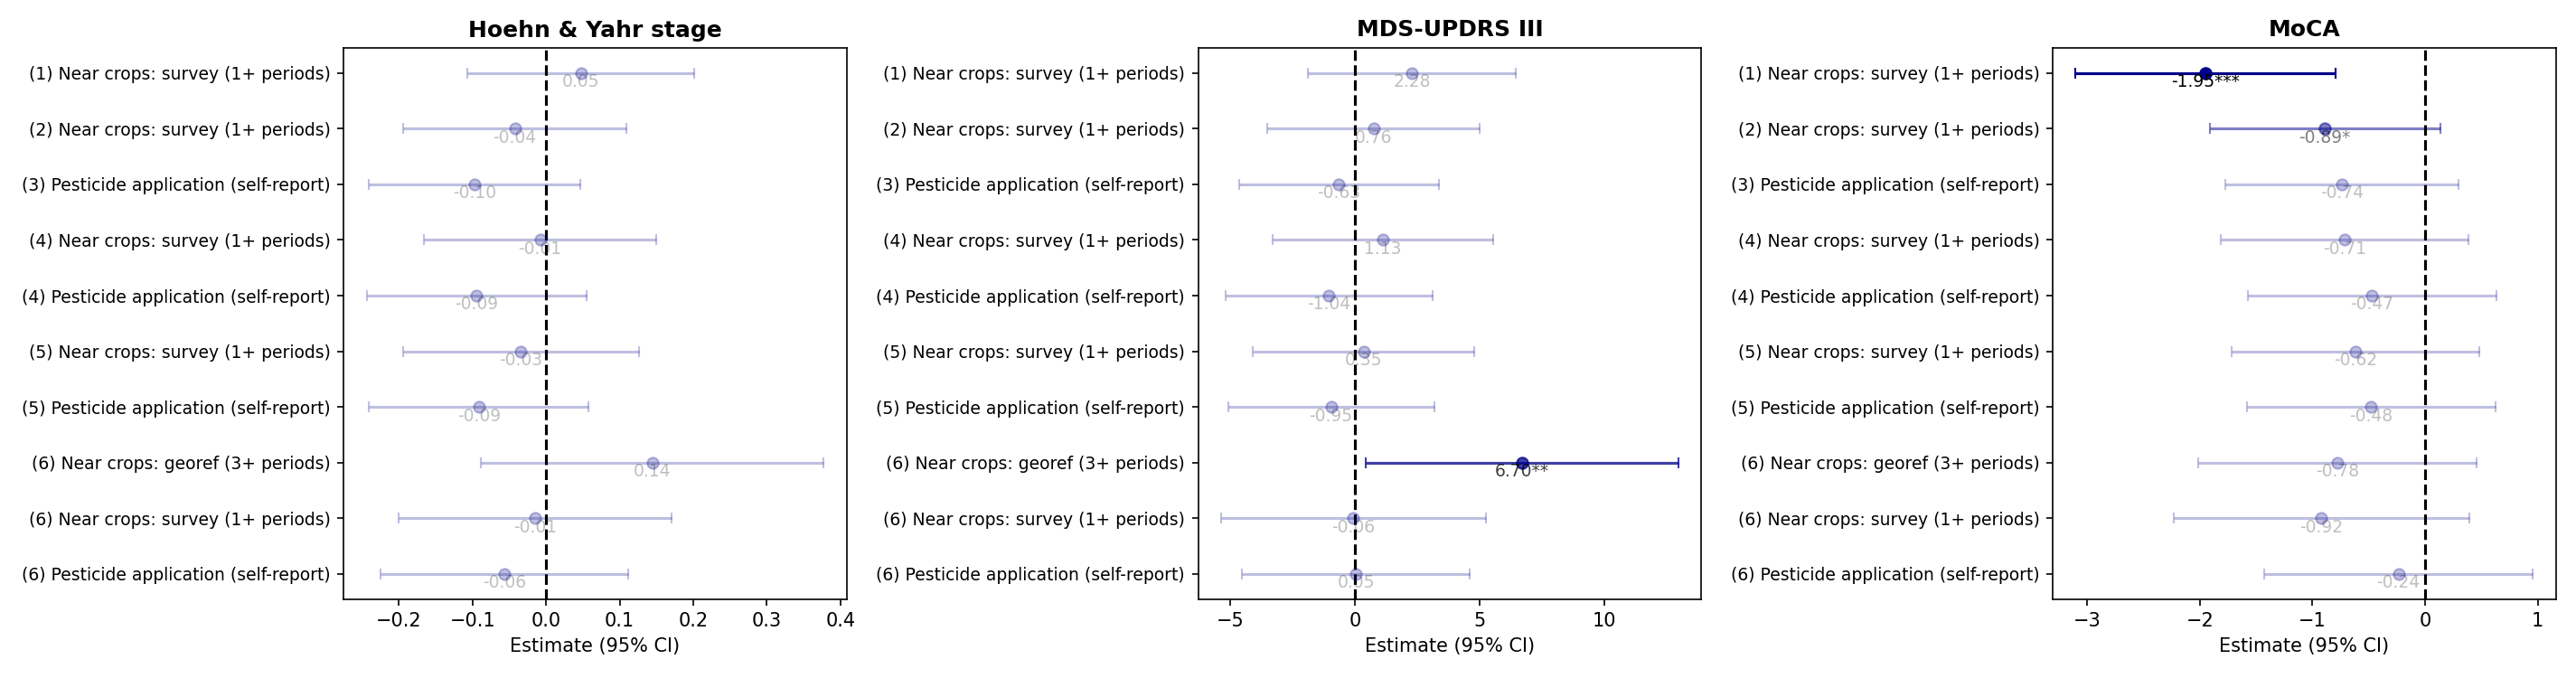
\includegraphics[width=\textwidth]{figures/coef_exposure.png}
\caption{Exposure coefficients with 95\% confidence intervals from the six specifications of Tables~\ref{tab:hy}, \ref{tab:updrs} and \ref{tab:moca} (column number in parentheses). Point shading marks significance (darkest $p<0.01$, lightest not significant).}\label{fig:coef}
\end{figure}

\subsection{Robustness of the survey estimate}

Table~\ref{tab:robust} re-estimates the survey coefficient of column (5) under six changes. Dropping levodopa gives $0.01$ stages, $0.9$ UPDRS points and $-0.7$ MoCA points. Dropping the 26 patients with an imputed disease duration gives $0.01$ stages, $1.8$ UPDRS points and $-0.6$ MoCA points. The linear count of periods near crops gives $-0.01$ stages, $0.0$ UPDRS points and $-0.2$ MoCA points per period (SE 0.03, 0.8 and 0.2). Cumulative years near crops gives $-0.01$ stages, $-0.1$ UPDRS points and $-0.1$ MoCA points per ten years (SE 0.02, 0.5 and 0.1). Restricting the sample to the 291 patients whose rural class comes from the map gives $0.01$ stages, $1.6$ UPDRS points and $-0.8$ MoCA points (SE 0.09, 2.3 and 0.6). An ordered logit for the staging scale gives $-0.05$ on the latent scale (SE 0.25). Every interval includes zero and none is wider than the baseline in substantive terms.

\begin{table}[H]\centering\scriptsize
\caption{Survey proxy coefficient under alternative specifications}\label{tab:robust}
\begin{tabular}{lcccc}
\hline\hline
Specification & Hoehn \& Yahr stage & MDS-UPDRS III & MoCA & N \\
\hline
Baseline, column (5) & -0.034 (0.082) & 0.352 (2.259) & -0.620 (0.562) & 346 \\
Without levodopa & 0.007 (0.086) & 0.906 (2.313) & -0.651 (0.558) & 346 \\
Dropping 26 patients with imputed duration & 0.011 (0.086) & 1.785 (2.348) & -0.615 (0.568) & 320 \\
Linear period count (per period) & -0.006 (0.027) & -0.025 (0.809) & -0.188 (0.174) & 346 \\
Linear years near crops (per 10 years) & -0.009 (0.017) & -0.061 (0.529) & -0.135 (0.117) & 346 \\
Geocoded residences only (DANE class) & 0.013 (0.092) & 1.552 (2.343) & -0.801 (0.595) & 291 \\
Ordered logit (latent scale) & -0.054 (0.246) &  &  & 346 \\
\hline\hline
\textit{Note:} & \multicolumn{4}{r}{Survey proxy coefficient (SE). HC1 SE; ordered logit conventional.} \\
\end{tabular}

\end{table}

\subsection{Number of life periods near crops}

Table~\ref{tab:periods} compares patients who reported living near crops in one, two, or three or more life periods with those who never did. Mean UPDRS is 31.1 for never, 30.5 for one period, 37.1 for two and 34.6 for three or more (Welch p-values 0.2 to 0.8); the staging scale is 2.1 to 2.3 throughout. Mean MoCA falls from 20.8 for never to 20.0, 19.8 and 17.6 for three or more periods (Welch $p=0.001$ for the last). With the full set of controls and rural residence (Table~\ref{tab:dummies}) the differences are $-1.3$ (SE 2.5), $3.2$ (SE 5.0) and $1.2$ (SE 3.7) UPDRS points, $-0.07$, $0.03$ and $-0.01$ stages, and $-0.4$ (SE 0.6), $0.3$ (SE 1.2) and $-1.2$ (SE 0.8) MoCA points; the raw cognitive gap of the three-or-more group is mostly its lower schooling. The share reporting pesticide handling rises from 17\% among the never-exposed to 71\% among those reporting three or more periods, and the share the map places near crops from 9\% to 56\%.

\begin{table}[H]\centering\scriptsize
\caption{Outcomes by number of life periods reported near crops, against patients who always answered "no" (Welch t-test p-values)}\label{tab:periods}
\begin{tabular}{lccccccccc}
\hline\hline
Periods (survey) & N & H\&Y & p vs 0 & UPDRS III & p vs 0 & MoCA & p vs 0 & Pesticide & Georef 3+ \\
\hline
0 & 255 & 2.15 &  & 31.1 &  & 20.8 &  & 0.17 & 0.09 \\
1 & 36 & 2.12 & 0.843 & 30.5 & 0.818 & 20.0 & 0.254 & 0.33 & 0.25 \\
2 & 13 & 2.31 & 0.360 & 37.1 & 0.228 & 19.8 & 0.456 & 0.54 & 0.20 \\
3+ & 42 & 2.21 & 0.549 & 34.6 & 0.315 & 17.6 & 0.001 & 0.71 & 0.56 \\
\hline\hline
\end{tabular}

\end{table}

\begin{table}[H]\centering\scriptsize
\caption{Adjusted differences by number of survey periods near crops (reference: never): OLS}\label{tab:dummies}
\begin{tabular}{lccc}
\hline\hline
 & Hoehn \& Yahr stage & MDS-UPDRS III & MoCA \\
 & (1) & (2) & (3) \\
\hline
Near crops in 1 period (survey) & -0.073 & -1.272 & -0.401 \\
 & (0.103) & (2.517) & (0.642) \\
Near crops in 2 periods (survey) & 0.027 & 3.177 & 0.312 \\
 & (0.161) & (4.983) & (1.151) \\
Near crops in 3+ periods (survey) & -0.011 & 1.224 & -1.236 \\
 & (0.117) & (3.710) & (0.831) \\
Pesticide application (self-report) & -0.100 & -1.282 & -0.373 \\
 & (0.077) & (2.145) & (0.585) \\
Rural residence (DANE class) & 0.288$^{*}$ & 8.564 & -0.965 \\
 & (0.155) & (5.307) & (1.198) \\
Age (years) & 0.009$^{***}$ & 0.136 & -0.091$^{***}$ \\
 & (0.003) & (0.086) & (0.025) \\
Female & -0.094 & -3.717$^{**}$ & -0.663 \\
 & (0.068) & (1.857) & (0.480) \\
Education (years) & -0.027$^{***}$ & -0.431$^{***}$ & 0.389$^{***}$ \\
 & (0.006) & (0.156) & (0.043) \\
Years since first symptom & 0.033$^{***}$ & 0.275 & -0.016 \\
 & (0.009) & (0.227) & (0.053) \\
Duration imputed (flag) & -0.049 & -0.206 & -0.104 \\
 & (0.121) & (3.614) & (1.162) \\
Ever drank coffee & -0.092 & -0.047 & 1.250 \\
 & (0.133) & (3.274) & (1.074) \\
Coffee intake (0--4 scale) & 0.046 & 1.192 & -0.161 \\
 & (0.046) & (1.138) & (0.244) \\
Ever smoked & -0.061 & -3.687$^{*}$ & -0.222 \\
 & (0.085) & (2.236) & (0.548) \\
Pack-year index & 0.013$^{**}$ & 0.199 & 0.001 \\
 & (0.006) & (0.146) & (0.028) \\
Levodopa treatment & 0.361$^{***}$ & 4.822$^{**}$ & -0.326 \\
 & (0.075) & (1.988) & (0.515) \\
\hline
Observations & 346 & 346 & 333 \\
Adjusted R$^2$ & 0.210 & 0.060 & 0.315 \\
\hline\hline
\textit{Note:} & \multicolumn{3}{r}{$^{*}$p$<$0.1; $^{**}$p$<$0.05; $^{***}$p$<$0.01. Robust SE (HC1).} \\
 & \multicolumn{3}{r}{Reference: never near crops.} \\
\end{tabular}

\end{table}

\subsection{Map-based comparison}

Table~\ref{tab:dose} tabulates severity by the number of periods the map places a geocoded patient within 500~m of cultivated land. Mean UPDRS rises from 30 with no periods to 38 with four and 44 with five, and mean MoCA falls from 21 to 18; the share reporting pesticide handling does not rise with either. In the regression of column (6) the three-period rule gives 6.7 points (SE 3.2, $p=0.04$), a one-period rule gives 4.7 points (SE 2.4, $p=0.05$), and the linear count gives 1.8 points per period (SE 0.8, $p=0.02$); the staging scale and the MoCA show no association under any rule (MoCA: $-0.8$, $0.0$ and $-0.1$ points, SE 0.6, 0.6 and 0.2). The two proxies thus behave in different ways: the survey count tracks pesticide handling, the map count tracks the raw motor means, and the map association holds with rural residence in the model.

\begin{table}[H]\centering\small
\caption{Severity and pesticide handling by number of life periods the map places within 500~m of cultivated land, geocoded patients}\label{tab:dose}
\begin{tabular}{lccccc}
\hline\hline
Periods near crops (georef) & N & Mean H\&Y & Mean UPDRS III & Mean MoCA & Pesticide share \\
\hline
0 & 197 & 2.11 & 29.7 & 21.0 & 0.20 \\
1 & 32 & 2.27 & 34.6 & 21.2 & 0.19 \\
2 & 17 & 2.15 & 31.5 & 19.3 & 0.47 \\
3 & 7 & 2.36 & 32.9 & 18.7 & 0.00 \\
4 & 22 & 2.23 & 37.9 & 18.1 & 0.50 \\
5 & 17 & 2.50 & 43.5 & 18.7 & 0.29 \\
\hline\hline
\end{tabular}

\end{table}

\section{Limitations}

The estimates require a valid proxy and conditional independence. The proxy is valid in the sense that patients who report living near crops are more likely to have been exposed than those who do not, and its count rises with pesticide handling and mapped proximity as expected. The share of proxy-positive patients who were in fact exposed remains unknown. If that share is low the estimate is a diluted version of the exposure effect, and a null on the proxy is compatible with a real effect of exposure. Quantifying the dilution requires an exposure measure, so the confidence intervals bound the effect of living near crops; the effect of pesticides themselves lies outside them.

Conditional independence is the assumption most at risk. Living near crops is a marker of rural birth, lower schooling and agricultural employment, and the sample is a clinic-and-brigade cohort drawn by referral and outreach. The cabecera class is a coarse proxy for access to care. It is held by 19 patients, so its coefficient has a standard error of five UPDRS points; it says nothing about travel time from a municipal seat to the specialist centre, and Tumaco, which contributes over forty patients to the cohort and has no specialist neurological service, counts as urban. For 55 patients the class comes from the address text, and an address that names no village is assumed urban. Rural disadvantage that the class leaves unmeasured, such as delayed treatment optimisation, would bias the proxy estimate upward if it raised severity, which strengthens the credibility of the null on the survey proxy. The same disadvantage remains a competing explanation for the map estimate and for the rural coefficient itself.

Measurement error differs between the proxies. The survey depends on recall of a "crop field", which a patient may define narrowly; this misclassification biases the estimate toward zero and could hide a small effect. The map depends on free-text geocoding with a municipal-centroid fallback, so many coordinates are town centres; 426 of 1,860 addresses did not resolve, 54 patients of the analytic sample have no map measure, and land-cover maps from 2005 and 2018 are applied to residences going back to the 1950s. A map hit and a survey "yes" coincide for about a quarter of the patients flagged by either. For these reasons the map result is reported as a comparison. The outcome carries error of its own: the medication state at the motor examination was not recorded, so patients examined in the ON and OFF states are pooled, which adds noise to the score and attenuates every association with it. Age at onset is also self-reported and carries entry error; the survey estimate is the same with and without the 26 patients whose duration is imputed.

Precision is limited. With 91 exposed patients the study can detect, at 80\% power, an effect of about 6.3 MDS-UPDRS III points (four tenths of a standard deviation), about 0.23 Hoehn \& Yahr stages and about 1.6 MoCA points (a third of a standard deviation). The intervals of $-4.1$ to $4.8$ UPDRS points, $-0.19$ to $0.13$ stages and $-1.7$ to $0.5$ MoCA points exclude moderate and large effects of the proxy but not small ones. The MoCA is a screening instrument graded by schooling and by age; it is adjusted for both, but any residual education effect that the linear years term misses would be attributed to the exposure, which is less educated. The design is cross-sectional: severity is observed once, at enrolment, so a higher level at a given disease duration is compatible with faster progression, earlier onset or later diagnosis.

\section{Discussion}

On the patients' own account of where they lived, residence within 500~m of a crop field in one, two, or three or more life periods is not associated with the Hoehn \& Yahr stage, the MDS-UPDRS III score or the MoCA score once age, sex, education, disease duration, coffee, smoking, levodopa and rural residence are held fixed. The same holds for the linear count of periods, for cumulative years near crops, for the patients whose rural class comes from the map alone, and for the patients' account of having applied or mixed pesticides. The raw motor means rise and the raw MoCA means fall with the number of periods near crops, and both gradients are explained by the lower education and the rural residence of the exposed. Effects larger than about five UPDRS points or two MoCA points are unlikely on this evidence; smaller effects are not excluded, and recall error, pooling of medication states and dilution of the proxy all work against detecting them.

The map-based proxy gives a different picture. Patients whom the geocoded residences place within 500~m of cultivated land in three or more periods score about seven MDS-UPDRS III points higher with a standard error of about three, the raw means rise with the number of mapped periods, and the one-period rule and the linear count of mapped periods reach or approach conventional significance. The direction is consistent with the Californian residential-proximity studies \citep{costello_parkinson_2009,li_proximity_2023} and with an ambient pathway, though the Dutch study found no such association for the same compounds \citep{brouwer_environmental_2017}. It is equally consistent with an access-to-care pathway: diagnostic latency in the LARGE-PD cohorts is long and varies by country \citep{ramchandra_sex_2025}, rural residents make fewer specialist visits where this has been measured \citep{crighton_patterns_2024}, and mapped proximity is itself a marker of rurality. Residence outside a cabecera carries its own nine points with the map proxy in the model, so the two markers are not the same thing, but the cabecera class is too coarse and too rare to settle whether the map association is exposure or distance from care. The data cannot separate the two.

The causal question therefore remains open. If the survey is the better measure, as its completeness and its correlates suggest, living near crops does not go with a worse motor examination in this cohort and the rural severity gap is better read as an access effect. If the map captures an ambient exposure that patients do not recognise as "living near a crop field", an environmental component co-occurs with access barriers in the same municipalities, as Rothman's sufficient-component model allows \citep{rothman_causes_1976,ritz_pesticides_2016}, and the survey null is a measurement failure.

Two descriptive patterns are worth recording. First, education and rural residence account for the raw association: the unadjusted survey estimate of 2.3 UPDRS points falls to 0.8 once education enters and to 0.4 once rural residence enters; each year of schooling is associated with about four tenths of a point less on the motor examination, 0.03 fewer stages and four tenths of a point more on the MoCA, survey-exposed patients have two fewer years of it, and residence outside a cabecera is associated with 8.8 more UPDRS points and 0.29 more stages. The MoCA is the outcome where education matters most: it accounts for about two thirds of the raw two-point cognitive gap between exposed and unexposed patients. The motor gradient by schooling matches the imaging cohort of Kotagal and colleagues, who report that ``higher educational attainment is associated with lower severity of motor impairment in PD'' \citep{kotagal_educational_2015}; whether it reflects motor reserve, better access to treatment among the more educated, or the coincidence of schooling and rural residence in this population, the data do not say. Second, the map proxy behaves like a rurality marker: it disagrees with the survey for most patients, is unrelated to pesticide handling, and its association with severity is of the same order as that of residence outside a cabecera.

Two improvements would make a decisive test possible: geocoding every residence to the house, so that the two proxies can be reconciled patient by patient and the cabecera class rests on the map for every patient, and adding a travel-time-to-care layer so that access can be controlled directly, including for municipal seats such as Tumaco that are urban but remote. Recording the medication state at examination would remove a source of outcome noise at no cost. If mapped proximity still predicted severity while reported proximity did not, the ambient interpretation would gain support and patients with sustained crop-adjacent residence would warrant earlier specialist review through the brigade programme. Until then, the evidence from this cohort is that living near crops, as patients report it, is not detectably associated with a worse motor examination or a lower cognitive score, that a moderate or large effect of that proxy can be ruled out, and that a small one cannot.

\bibliographystyle{unsrtnat}
\bibliography{references}

\end{document}
